\documentclass[a4paper,12pt,oneside]{book}

\usepackage[T1]{fontenc}
\usepackage[utf8]{inputenc}
\usepackage[italian]{babel}
\usepackage{pifont}
\usepackage{enumitem}
\usepackage[colorlinks]{hyperref}
\usepackage{graphicx} % Required for inserting images
\usepackage{geometry}
\usepackage{soul}
\usepackage{titlepic}
\usepackage{mdframed}
\usepackage{booktabs}
\sethlcolor{blue}
\hypersetup{
    hidelinks,
    colorlinks=true,
    linkcolor=black,      
    pdftitle={Documentazione Galleria Condivisa},
    pdfpagemode=FullScreen,
}
\geometry{a4paper, top = 3cm, bottom = 3cm, left = 3.5cm, right = 3.5cm, heightrounded, bindingoffset = 5mm}
\pagestyle{plain}

\title{\textrm{Documentazione\\Galleria Fotografica Geolocalizzata}}
\author{Gennaro Ventrone\and Luigi Solaro\and Mariano Sommella}
\date{\textsc{\large anno accademico 2022-2023}}



\setcounter{secnumdepth}{3}
\setcounter{tocdepth}{2}

\begin{document}       
    \titlepic{
\includegraphics[width=.25\textwidth]{FedericoII.png}}
    \begin{titlepage}
        \maketitle
    \end{titlepage}
    
        \frontmatter
        \tableofcontents
        \mainmatter
        
    \chapter{Specifiche Progetto}
    
    \section{Introduzione Documentazione}
    \par
    Nelle seguenti pagine si riporta la documentazione relativa ad una progettazione e implementazione di un sistema di basi di dati per la gestione di collezioni fotografiche geolocalizzate condivise.\par \paragraph{
    \footnotesize Per una visione migliore del documento si utilizzi l'indice e le varie sezioni menzionate.}
    
    \section{Elenco Specifiche}
   Vengono qui elencate le caratteristiche che l'applicativo deve garantire:
    \begin{enumerate}
        \item \emph{Informazioni sulla foto:} Possibilità di visualizzare per ogni foto l'utente che l'ha scattata, il dispositivo utilizzato e il luogo in cui è stata scattata. Il luogo può essere identificato da coordinate geografiche o da un nome mnemonico unico all'interno del sistema.
        
        \item \emph{Identificazione dei soggetti:} Ogni foto può raffigurare diversi soggetti o utenti, in entrambi i casi devono essere identificati univocamente e categorizzati.

        \item \emph{Accesso a collezioni fotografiche:} Ogni utente ha sempre la possibilità di vedere la propria galleria fotografica personale, che comprende esclusivamente le foto scattate da lui. Un utente può partecipare a collezioni condivise con altri utenti che possono contenere foto scattate da questi ultimi. 
        
         \item \emph{Accesso alla foto:} Ogni utente deve avere la possibilità di accedere solo alle proprie foto o a quelle condivise con gli altri utenti. Le foto private non verranno condivise con gli altri utenti.
         
        \item \emph{Eliminazione delle foto:} Gli utenti devono avere la possibilità di eliminare le proprie foto, ma solo l'amministratore del sistema può eliminare un utente e tutte le sue foto (eccetto le fotografie che contengono come soggetto un altro utente).

        \item \emph{Operazione di ricerca:} Il sistema deve permettere la ricerca di foto in base al luogo in cui sono state scattate o al soggetto rappresentato. Inoltre, deve essere possibile visualizzare una classifica dei 3 luoghi più immortalati.
        \item \emph{Gestione dei video:} Ogni fotografia può essere visualizzata in sequenza, andando a formare quindi un video. %(sezione)

        \item \emph{Sicurezza:} Il sistema deve garantire la sicurezza delle informazioni, in particolare la gestione degli account degli utenti e la protezione dei dati personali. Inoltre, il sistema deve essere in grado di gestire la concorrenza tra utenti per evitare problemi di accesso simultaneo alle stesse informazioni.
    \end{enumerate}
    \par
    
    Il sistema prevede che le categorie di utenti siano così rappresentate:
    \begin{itemize}
        \item \textbf{Utente:} Può effettuare i punti dal 1 al 7 (In particolare esiste un servizio riservato al ruolo di \emph{amministratore} nel punto 5).

        \item \textbf{Soggetto:} Può essere ritratto e taggato in una fotografia ed essere categorizzato.

        \item \textbf{Amministratore:} Può effettuare il punto 5 e avere accesso agli stessi servizi di \emph{Utente}.
    \end{itemize} 
    \chapter{Modello Concettuale}
    \section{Passaggio dal minimondo al modello concettuale}\par
    Il \emph{mini-world} è una rappresentazione semplificata del mondo reale che ci fa intuire le informazioni che devono essere salvate nel database.
    Superata la prima fase che consiste quindi nella raccolta e analisi dei requisiti, la seconda fase consiste nel tradurre questi ultimi in entità e relazioni mediante un costrutto grafico.
    In seguito alla sezione precedente si è costruito il seguente schema concettuale espresso mediante il Diagramma UML:
    
    \section{Ristrutturazione del modello concettuale}
      La terza fase della progettazione di un sistema di basi di dati consiste nel passaggio dal modello concettuale al modello logico. La ristrutturazione del modello concettuale è un processo che si occupa di migliorare il modello concettuale, in questo caso quello precedentemente realizzato, per renderlo più efficiente e aggiornato alle esigenze degli utenti. Può essere realizzato nel seguento modo:

      \iffalse
      \begin{figure}
          \centering         \includegraphics{C:/Users/user/Pictures/miafoto}
          \caption{Caption}
          \label[width=0.7\linewidth]{fig:my_label}
      \end{figure}
      \fi
    \subsection{Analisi delle ridondanze}
    Le ridondanze sono costituite da dati ricavabili tramite operazioni da altri dati presenti nello schema. Nel modello realizzato precedentemente non sono presenti ridondanze, tuttavia introduciamo tre attributi derivati:
    \begin{enumerate}

         \item\texttt{Collezione.\textbf{numero\textunderscore elementi}}
         \item\texttt{Video.\textbf{numero\textunderscore frames}}
         \item\texttt{Video.\textbf{durata}}


    \end{enumerate}
    Notiamo che essi sono ridondanti in quanto \texttt{collezione.numero\textunderscore elementi} e \texttt{video.numero\textunderscore frames} che corrispondono al numero d'istanze di associazione di tipo \textbf{contenuto} e \textbf{contenuto video} per una certa collezione o video, mentre \texttt{video.durata} corrisponde alla somma delle durate di tutti i frame contenuti in un certo video.
    Andremo a implementare in modo  efficiente tali attributi tramite i trigger presenti nella \textsc{sezione \ref{sec:Intro}}

    \subsection{Analisi delle Generalizzazioni}
    In un modello di dati, una relazione di generalizzazione/specializzazione rappresenta un'entità generica (superclasse) che ha una o più sottoclassi (entità specializzate) con attributi specifici aggiuntivi. Nel modello concettuale realizzato sono presenti due istanze di specializzazione, ovvero \texttt{Admin->Utente} e \texttt{Soggetto->Utente}. Decidiamo di accorpare \texttt{Admin} nell'entità padre come attributo Booleano, mentre sostituiamo la generalizzazione di \texttt{Soggetto} con l'associazione all'entità padre.
    
    \subsection{Rimozione di Attributi Multivalori e Composti}
    Gli attributi multivalore sono attributi che possono contenere più di un valore per ogni tupla, mentre gli attributi composti sono attributi che contengono al loro interno più di un sotto-attributo o campo dati. Nel modello concettuale è presente solo un attributo composto, ovvero \texttt{coordinate(Latitudine, Longitudine)}. Per ristrutturarlo scomponiamo \texttt{coordinate} rendendo i due sotto-attributi in due attributi indipendenti.
    
    \subsection{Analisi di Entità e Associazioni}
    L'analisi delle Entità e Associazioni prevede di valutare i requisiti del sistema e l'attuale modello del database per identificare eventuali problemi di progettazione o inefficienze. Nel modello concettuale, Video è espresso come composizione di \texttt{frame}. Ristrutturiamo l'associazione come associazione identificante e \texttt{frame} come entità debole di \texttt{Video}.
    
    \subsection{Analisi degli Identificativi}
    Una chiave primaria è un attributo o un insieme di attributi che identifica univocamente ogni tupla di una tabella del database. Elenchiamo gli identificativi per ogni entità:\par
    \begin{itemize}
        \item \textbf{Fotografia:} La traccia richiede che ogni fotografia sia identificata univocamente, introduciamo quindi \texttt{id\textunderscore foto}.
        
        \item \textbf{Luogo:} Quanto richiesto, il sistema permette di identificare un luogo tramite le coordinate geografiche, scegliamo come chiave primaria gli attributi \texttt{Latitudine} e \texttt{Longitudine}.
        
        \item \textbf{Collezione:} Viene specificato che l'applicativo debba permettere ad ogni utente di accedere a gallerie condivise da altri utenti, pertanto si è scelto di aggiungere l'identificativo \texttt{id\textunderscore collezione}, in quanto gli attributi presenti nella tabella potrebbero essere inefficienti.
        
        \item \textbf{Utente:} Scegliamo \texttt{username} come chiave primaria.
        \item \textbf{Soggetto:} Scegliamo \texttt{nome} come chiave primaria.
        \item \textbf{Video:} Introduciamo l'identificante \texttt{id\textunderscore video} seguendo la stessa logica adottata per l'entità \texttt{Video}.
        \item \textbf{Frame:} L'entità \texttt{Frame} essendo un'entità debole non ha un identificatore primario, abbiamo trovato opportuno utilizzare \texttt{ordine} come chiave parziale.
    \end{itemize}
    
    \section{Diagramma Ristrutturato}
    \subsection{Diagramma ER}
    
    \subsection{Diagramma UML}
    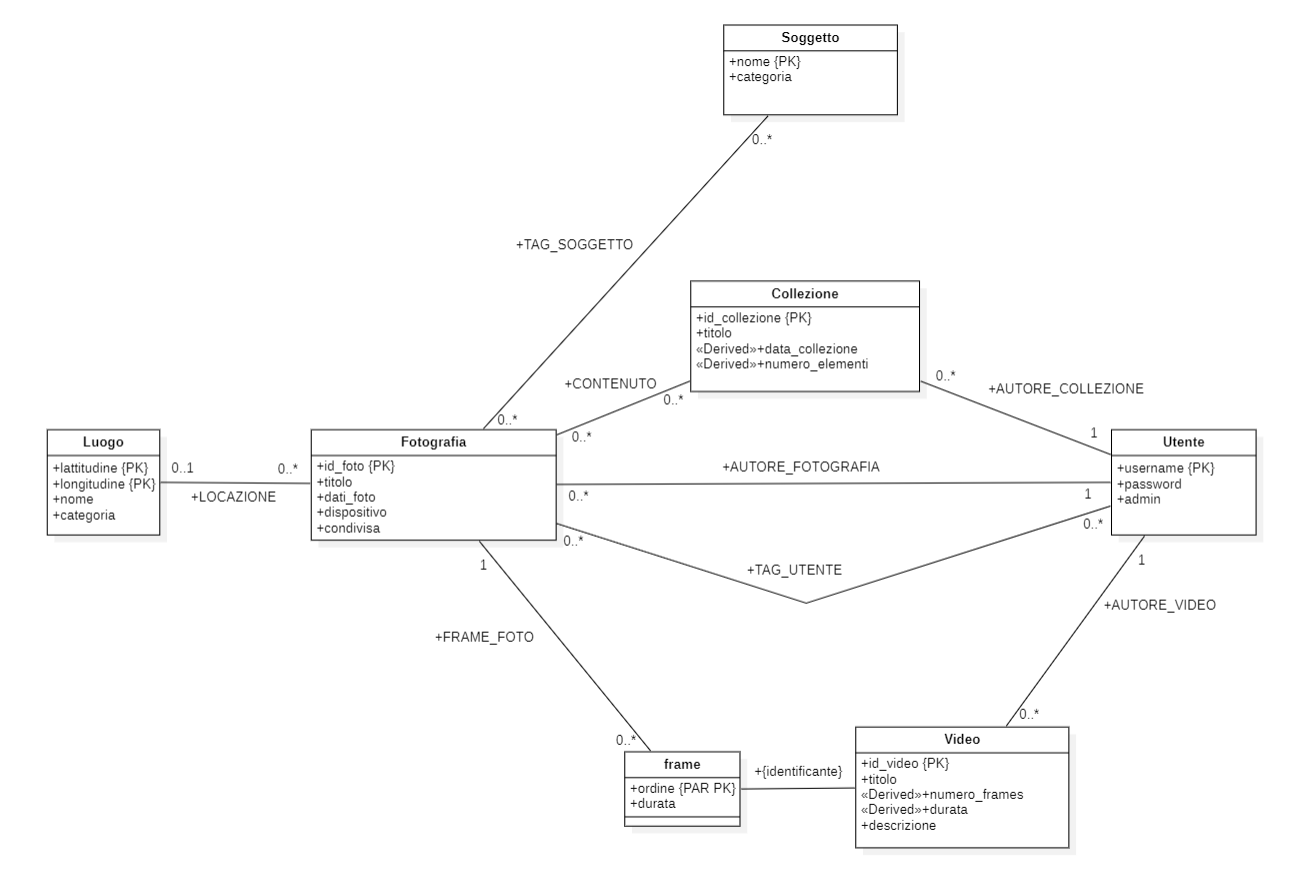
\includegraphics[scale=0.50]{UML.png}
    
    \section{Dizionario delle Entità}
  
    \section{Dizionario delle Associazioni}
    \section{Dizionario dei Vincoli}

    \chapter{Progettazione Logica}
    \section{Passaggio dal Diagramma ER al Modello Logico}
    \section{Mapping delle Entità e delle Associazioni}
    \section{Schema Logico}
    \chapter{Codice SQL}
    \section{Definizioni preliminari}
    \section{Creazioni Tabelle}
\par Vengono presentate qui in questa sezione i codici delle relative tabelle tradotte precedentemente dal modello logico.\par
\vspace{2cm}


\texttt{1} \textbf{CREATE TABLE IF NOT EXISTS} \texttt{utente (}\par
\texttt{2\qquad username} \textbf{VARCHAR(30) NOT NULL},\par
\texttt{3\qquad password} \textbf{VARCHAR(30) NOT NULL},\par
\texttt{4\qquad admin} \textbf{BOOLEAN NOT NULL DEFAULT false},\par
\texttt{5}\qquad \textbf{CONSTRAINT} \texttt{utente}\textunderscore pk \textbf{PRIMARY KEY} \texttt{(username)}\par
\texttt{6 );}

\vspace{1cm}

\texttt{1} \textbf{CREATE TABLE IF NOT EXISTS} \texttt{luogo (}\par
\texttt{2\qquad	latitudine} \textbf{FLOAT NOT NULL},\par
\texttt{3\qquad	longitudine} \textbf{FLOAT NOT NULL},\par
\texttt{4\qquad	nome} \textbf{VARCHAR(50) UNIQUE},\par
\texttt{5\qquad	descrizione} \textbf{VARCHAR(225)},\par
\texttt{6}\qquad	\textbf{CONSTRAINT} \texttt{luogo\textunderscore pk} \textbf{PRIMARY KEY} \par \qquad \texttt{(latitudine, longitudine)}\par
\texttt{7 );}

\vspace{1cm}

\texttt{1} \textbf{CREATE TABLE IF NOT EXISTS} \texttt{nometabella (}\par
\texttt{indice \qquad nomeattributo} \textbf{tipodidato}, \par
\texttt{indice} \qquad \textbf{CONSTRAINT} \texttt{nome \textunderscore pk} \textbf{PRIMARY FOREIGN KEY} \par \qquad \texttt{nomeattributo} \par
\texttt{indice );}
    \section{View}
    \section{Trigger}
    \label{sec:Intro}
\end{document}
